\documentclass{article}

% - Style
\usepackage{base}

% - Plotting
\usepgfplotslibrary{units}
\usepackage{pgfplotstable}

% - Listings
\usepackage{color}
\usepackage{listings}

\lstset{
  basicstyle=\ttfamily\footnotesize\color{black}
  , commentstyle=\color{blue}
  , keywordstyle=\color{purple}
  , stringstyle=\color{orange}
  %
  , numbers=left
  , numbersep=5pt
  , stepnumber=1
  , numberstyle=\ttfamily\small\color{black}
  %
  , keepspaces=true
  , showspaces=false
  , showstringspaces=false
  , showtabs=false
  , tabsize=2
  , breaklines=true
  %
  , frame=single
  , backgroundcolor=\color{white}
  , rulecolor=\color{black}
  , captionpos=b
}

% file or folder
\lstdefinestyle{ff}{
  basicstyle=\ttfamily\normalsize\color{orange}
}

% - Title
\title{PHYS4004 High Performance Computing - Assignment 2: MPI}
\author{Tom Ross - 1834 2884}
\date{}

% - Headers
\pagestyle{fancy}
\fancyhf{}
\rhead{\theauthor}
\chead{}
\lhead{\thetitle}
\rfoot{\thepage}
\cfoot{}
\lfoot{}

% - Document
\begin{document}

\tableofcontents

\newpage
\section{Overview}
\label{sec:overview}

The codebase \lstinline[style=ff]{mandelbrot}, which can be found at
\url{https://github.com/dgsaf/mandelbrot}, consists of the original code
provided by Associate Professor Nigel Marks, with the following additions:
\begin{itemize}
\item \lstinline[style=ff]{src/mandelbrot_static.f90}:

\item \lstinline[style=ff]{src/mandelbrot_master_worker.f90}:

\item \lstinline[style=ff]{src/mandelbrot_cyclic.f90}:

\item \lstinline[style=ff]{mandelbrot.slurm}:

\item \lstinline[style=ff]{mandelbrot-static.slurm}:

\item \lstinline[style=ff]{mandelbrot-master_worker.slurm}:

\item \lstinline[style=ff]{mandelbrot-cyclic.slurm}:

\item \lstinline[style=ff]{mandelbrot-jobs.sh}:

\item \lstinline[style=ff]{output/}:

\item \lstinline[style=ff]{bin/}:

\item \lstinline[style=ff]{pictures/}:

\end{itemize}

\newpage
\section{Serial}
\label{sec:serial}

The Mandelbrot serial code, \lstinline[style=ff]{src/mandelbrot.f90}, can be
found in \autoref{sec:serial-code}.

\newpage
\section{Static Decomposition}
\label{sec:static}

The Mandelbrot MPI static decomposition code,
\lstinline[style=ff]{src/mandelbrot_static.f90}, can be found in
\autoref{sec:static-code}.

% compare performance with serial code

% discuss load balance

% load balance graph
The load-balance for the 10 processes is show in
\autoref{fig:static-load-balance}.
\begin{figure}[h]
  \centering
  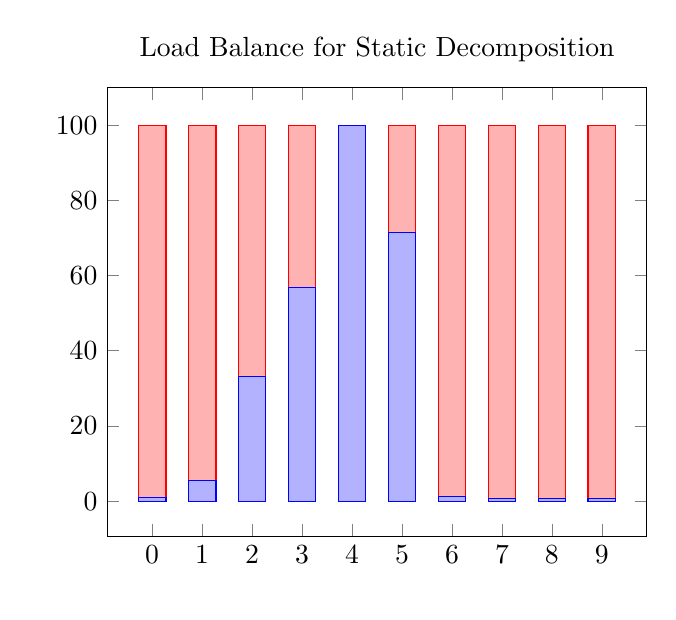
\begin{tikzpicture}
    \pgfplotstableread[col sep=comma, header=true]{
      process, working, waiting, communicating
      0,  0.91, 98.94, 0.15
      1,  5.42, 94.54, 0.03
      2, 33.25, 66.70, 0.05
      3, 56.85, 43.09, 0.06
      4, 99.92,  0.00, 0.08
      5, 71.39, 28.52, 0.09
      6,  1.21, 98.68, 0.11
      7,  0.78, 99.10, 0.12
      8,  0.68, 99.18, 0.14
      9,  0.60, 99.25, 0.15
    }\data

    \begin{axis}[
      ybar stacked
      , xtick={0, 1, ..., 9}
      , title={Load Balance for Static Decomposition}
      ]

      \addplot table[x=process, y=working] from \data;
      \addplot table[x=process, y=waiting] from \data;
      \addplot table[x=process, y=communicating] from \data;

    \end{axis}
  \end{tikzpicture}
  \caption{The load balance for the Mandelbrot MPI static decomposition scheme,
    with 10 processes, where $N = 8000$, $\mathrm{maxiter} = 1000$. For each
    process, the percentage of time spent working is shown in blue, the
    percentage of time spent waiting in red, and the percentage of time spent
    communicating is shown in brown (however, this time is negligble and so is
    barely visible).}
  \label{fig:static-load-balance}
\end{figure}

\newpage
\section{Master-Worker Scheme}
\label{sec:master-worker}

The Mandelbrot MPI master-worker scheme code,
\lstinline[style=ff]{src/mandelbrot_master_worker.f90}, can be
found in \autoref{sec:master-worker-code}.

% compare performance with static

% compare load balance with static (for chunksize = 100000)

% discuss how load balance varies with chunksize

% execution time graph vs chunksize

\newpage
\section{Cyclic Decomposition}
\label{sec:cyclic}

The Mandelbrot MPI cyclic decomposition code,
\lstinline[style=ff]{src/mandelbrot_cyclic.f90}, can be found in
\autoref{sec:cyclic-code}.

% compare performance with static

% discuss load imbalance

% discuss which is best strategy

\clearpage
\appendix
\section{Appendix}
\label{sec:appendix}

\newpage
\subsection{Serial}
\label{sec:serial-code}

\lstinputlisting[
language=Fortran
]{../src/mandelbrot.f90}

\newpage
\subsection{Static Decomposition}
\label{sec:static-code}

\lstinputlisting[
language=Fortran
]{../src/mandelbrot_static.f90}

\newpage
\subsection{Master Worker Scheme}
\label{sec:master-worker-code}

\lstinputlisting[
language=Fortran
]{../src/mandelbrot_master_worker.f90}

\newpage
\subsection{Cyclic Decomposition}
\label{sec:cyclic-code}

\lstinputlisting[
language=Fortran
]{../src/mandelbrot_cyclic.f90}


\end{document}